\documentclass[12pt,a4paper]{article}
\usepackage[latin1]{inputenc}
\usepackage[spanish]{babel}
\usepackage{amsmath}
\usepackage{amsfonts}
\usepackage{amssymb}
\usepackage{graphicx}
\usepackage[left=2cm,right=2cm,top=2cm,bottom=2cm]{geometry}
\author{MEJORADA LOPEZ IVAN}
\title{ARREGLOS Y PARAMETROS DE LOS AMPLIFICADORES CLASE A}
\begin{document}

\maketitle

\includegraphics[width=17.5cm]{UPZMG_Prueba_1b.png} 
\newpage
\section{AMPLIFICADORES DE CLASE (A)}
Amplificador clase A

Los amplificadores emisores comunes son el tipo de amplificador m\'as com\'unmente usado, ya que pueden tener una ganancia de voltaje muy grande.

Los amplificadores Common Emitter (CE) est\'an dise\~nados para producir una gran oscilaci\'on de voltaje de salida desde un voltaje de se\~nal de entrada relativamente peque\~no de solo unos pocos milivoltios y se usan principalmente como "amplificadores de peque\~na se\~nal" como vimos en los tutoriales anteriores.
\\
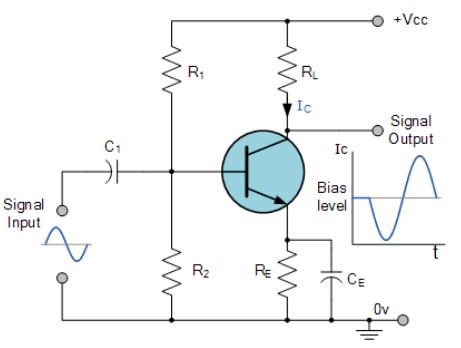
\includegraphics[width=10cm]{Amplificador clase A.jpg} 
\section{caracteristicas de los amplificadores clase A }
Esta amplificaci\'on presenta el inconveniente de generar una fuerte y constante emisi\'on de calor. No obstante, los transistores de salida est\'an siempre a una temperatura fija y sin alteraciones\\
En general, se afirma que esta clase de amplificaci\'on es frecuente en circuitos de audio y en los equipos dom\'esticos de gama alta, ya que proporcionan una calidad de sonido potente y de muy buena calidad.\\
Los amplificador de clase (A) a menudo consisten en un transistor de salida conectado al positivo de la fuente de alimentaci\'on y un transistor de corriente constante conectado de la salida al negativo de la fuente de alimentaci\'on.\\
\\
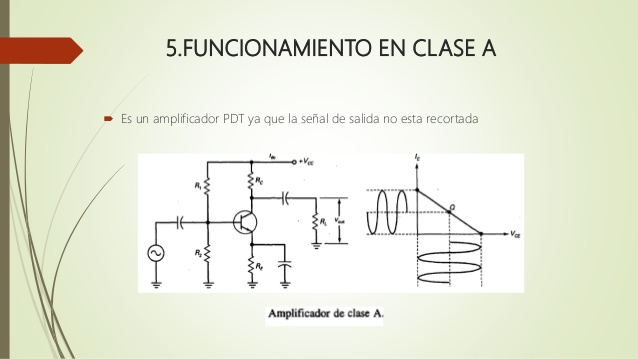
\includegraphics[width=10cm]{amplificadores-de-potencia-f-13-638.jpg}
\\
\section{FUNCION PRINCIPAL}La funci\'on principal del amplificador de potencia, que tambi\'en se conoce como "amplificador de se\~nal grande", es suministrar potencia, que es el producto del voltaje y la corriente de la carga. B\'asicamente, un amplificador de potencia tambi\'en es un amplificador de tensi\'on, con la diferencia de que la resistencia de carga conectada a la salida es relativamente baja, por ejemplo, un altavoz de 4 ohms o 8 ohms resulta en corrientes altas que fluyen a trav\'es del colector del transistor.

\section{VENTAJAS}
La clase A se refiere a una etapa de salida con una corriente de polarizaci\'on mayor que la m\'axima corriente de salida que dan, de tal forma que los transistores de salida siempre est\'an consumiendo corriente. La gran ventaja de la clase (A) es que es casi lineal, y en consecuencia la distorsi\'on es menor.\\
\section{DESVENTAJAS}
La gran desventaja de la clase A es que es poco eficiente, se requiere un amplificador de clase (A) muy grande para dar 50 W, y ese amplificador usa mucha corriente y se pone a muy alta temperatura.


 
 


\end{document}